\documentclass[10pt]{article}

\pagestyle{empty}

\setlength{\textheight}{250mm}
\setlength{\textwidth}{180mm}
\setlength{\oddsidemargin}{-8mm}
\setlength{\topmargin}{-1.5cm}

\usepackage{amsmath}
\usepackage{amsthm}
\usepackage{psfrag}
\usepackage{graphicx}
\usepackage{bm}
\usepackage{mathrsfs}
\usepackage{icomma} % pacchetto per limitare lo spazio standard posto dopo la virgola in caso che la virgola sia tra cifre
\usepackage{amsfonts} % amplia i caratteri matematici disponibili
\usepackage{amssymb}
%\usepackage{wrapfig}
\usepackage{empheq}

\usepackage{epstopdf}
\usepackage[utf8x]{inputenc}
\usepackage{ifthen}

\usepackage[italian]{babel}
%\usepackage[latin1]{inputenc}

%\include{def}

%\newcommand{\kg}{\textrm{kg}}
%\newcommand{\K}{\textrm{K}}
%\newcommand{\m} {\textrm{m}}
%\newcommand{\dm}{\textrm{dm}}
%\newcommand{\cm}{\textrm{cm}}
%\newcommand{\mm}{\textrm{mm}}
%\newcommand{\s} {\textrm{s}}
%\newcommand{\N} {\textrm{N}}
%\renewcommand{\Pa}{\textrm{Pa}}
%\newtheorem{exerciseS}{Esercizio}
\def \flagSect{0} % 1    : numerazione
		  % else : niente
%\newcommand{\taitol}[1]  % stile titolo
%{
%%{\textit{#1}}
%{#1}
%}
\def \soluzione{Soluzione}
\def \partePrima{Concetti. }
\def \parteSeconda{Svolgimento. }
%\def \parteTerza{}
\newcommand{\sol}{\subsubsection*{\soluzione}}
\newcommand{\partone}{\ \ \ \ \ \textbf{\partePrima}}
\newcommand{\parttwo}{\vspace{0.2cm}\textbf{\parteSeconda}}

\ifnum\flagSect=1
\newtheorem{esercizio}{Esercizio}%[section]
\else
\newtheorem*{esercizio}{Esercizio}
\fi

\newtheorem*{teorema}{Teorema}
\newtheorem*{lemma}{Lemma}

% ###########################################################
%\def \flagSect{0} % 1    : numerazione
		  % else : niente
%\newcommand{\taitol}[1]  % stile titolo
%{
%%{\textit{#1}}
%{#1}
%}
\def \soluzione{Soluzione}
\def \partePrima{Concetti. }
\def \parteSeconda{Svolgimento. }
%\def \parteTerza{}
\newcommand{\sol}{\subsubsection*{\soluzione}}
\newcommand{\partone}{\ \ \ \ \ \textbf{\partePrima}}
\newcommand{\parttwo}{\vspace{0.2cm}\textbf{\parteSeconda}}

\ifnum\flagSect=1
\newtheorem{esercizio}{Esercizio}%[section]
\else
\newtheorem*{esercizio}{Esercizio}
\fi

\newtheorem*{teorema}{Teorema}
\newtheorem*{lemma}{Lemma}

% ###########################################################
%\def \flagSect{0} % 1    : numerazione
		  % else : niente
%\newcommand{\taitol}[1]  % stile titolo
%{
%%{\textit{#1}}
%{#1}
%}
\def \soluzione{Soluzione}
\def \partePrima{Concetti. }
\def \parteSeconda{Svolgimento. }
%\def \parteTerza{}
\newcommand{\sol}{\subsubsection*{\soluzione}}
\newcommand{\partone}{\ \ \ \ \ \textbf{\partePrima}}
\newcommand{\parttwo}{\vspace{0.2cm}\textbf{\parteSeconda}}

\ifnum\flagSect=1
\newtheorem{esercizio}{Esercizio}%[section]
\else
\newtheorem*{esercizio}{Esercizio}
\fi

\newtheorem*{teorema}{Teorema}
\newtheorem*{lemma}{Lemma}

% ###########################################################
%\input{logicNumb}
%\newcommand{\sectionIf}[2]
%{
%   \ifthenelse{\equal{#1}{1}}
%              {\subsection{#2}}{\subsection*{#2}}
%}
% ###########################################################

%\newcommand{\sectionIf}[2]
%{
%   \ifthenelse{\equal{#1}{1}}
%              {\subsection{#2}}{\subsection*{#2}}
%}
% ###########################################################

%\newcommand{\sectionIf}[2]
%{
%   \ifthenelse{\equal{#1}{1}}
%              {\subsection{#2}}{\subsection*{#2}}
%}
% ###########################################################



\begin{document}

\begin{center}
\textbf{Esercizi per il corso di Fluidodinamica} 
\medskip
\end{center}


\noindent
\begin{tabular}{cc}
\begin{minipage}[b]{0.60\textwidth}
\begin{exerciseS}[Corrente di Poiseuille in un tubo a sezione circolare e manometro]
Un manometro a mercurio ($\rho_{hg} = 13610 \  kg/m^3$)
collega due prese di pressione posizionate a una distanza di $l = 2 \ 
m$ l'una dall'altra lungo un tubo orizzontale di diametro $2R = 5 \ cm$
 in cui scorre un fluido con densità $\rho_{f} = 950 \
kg/m^3$. Se la differenza fra le altezze dei peli liberi del 
liquido manometrico nelle due colonne
vale $\Delta h = 4 \ cm$ e la portata volumetrica che scorre nel tubo è 
$Q= 6\ m^3/s$,
quanto valgono la viscosità $\mu$ del fluido e lo sforzo a parete
$\tau_w$?

($\mu = 6.36\,10^{-5} \ kg/(m\, s)$,
$\tau_w = 31.05\, \bm{z}\ N/m^2$)
\end{exerciseS}
\end{minipage}
&
\begin{minipage}[b]{0.35\textwidth}
   \begin{center}
   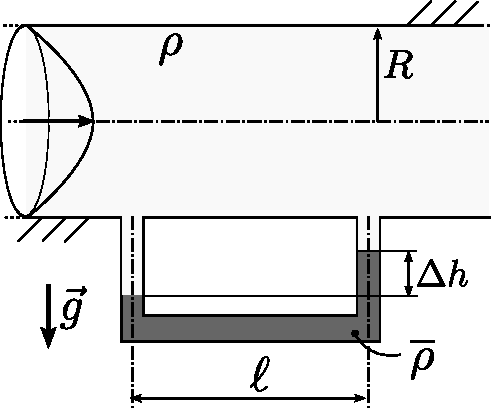
\includegraphics[width=0.90\textwidth]{./fig/slnEsatte-poiseuille}
   \end{center}
\end{minipage}
\end{tabular}


\sol

\partone Semplificazione delle equazioni di NS in casi particolari. 
Soluzioni esatte in coordinate cilindriche. Legge di Stevino.

Scrittura del contributo viscoso del vettore sforzo come:
\begin{equation}
\begin{aligned}
  \bm{s_n} & = \mathbb{S} \cdot \bm{\hat{n}} = \\
           & = \mu [\bm{\nabla} \bm{u} + \bm{\nabla}^T \bm{u}] \cdot \bm{\hat{n}} = \\
           & = \mu \left[ 2 (\bm{\hat{n}} \cdot \bm{\nabla} ) \bm{u} + \bm{\hat{n}} \times \bm{\nabla} \times \bm{u}  \right]
\end{aligned}
\end{equation}

\parttwo La geometria del problema suggerisce di utilizzare un sistema di coordiante cilindriche.

\begin{itemize}
  \item Scrittura delle equazioni di NS in coordinate cilindriche
  \begin{equation}
  \begin{cases}
    \rho \dfrac{\partial u_r}{\partial t}
    + \rho \left( \bm{u} \cdot \bm{\nabla}u_r - \dfrac{u_\theta^2}{r} \right)
    - \mu \left(\nabla^2 u_r 
       - \dfrac{u_r}{r^2} 
       - \dfrac{2}{r^2}\dfrac{\partial u_\theta}{\partial \theta} \right)  
       + \dfrac{\partial p}{\partial r} = f_r \\
    \rho \dfrac{\partial u_\theta}{\partial t}
    + \rho \left( \bm{u} \cdot \bm{\nabla} u_\theta + \dfrac{u_\theta u_r}{r} \right)
    - \mu \left(\nabla^2 u_\theta 
       - \dfrac{u_\theta}{r^2} 
       + \dfrac{2}{r^2}\dfrac{\partial u_r}{\partial \theta}  \right) 
    + \dfrac{1}{r} \dfrac{\partial p}{\partial \theta} = f_\theta\\
    \rho \dfrac{\partial u_z}{\partial t}
    + \rho \bm{u} \cdot \bm{\nabla} u_z
    - \mu \nabla^2 u_z
    + \dfrac{\partial p}{\partial z} = f_z \\ \\
    \dfrac{1}{r}\dfrac{\partial}{\partial r}\left( r u_r \right) 
    + \dfrac{1}{r}\dfrac{\partial u_\theta}{\partial \theta} 
    + \dfrac{\partial u_z}{\partial z} = 0
  \end{cases}
  \end{equation}
  con 
  \begin{equation}
  \begin{aligned}
  & \bm{a} \cdot \bm{\nabla} b = a_r \dfrac{\partial b}{\partial r} 
     + \dfrac{a_\theta}{r} \dfrac{\partial b}{\partial \theta}  
     + a_z \dfrac{\partial b}{\partial z} \\
  & \nabla^2 f = \dfrac{1}{r}\dfrac{\partial}{\partial r}
                      \left(r \dfrac{\partial f}{\partial r} \right) +
               \dfrac{1}{r^2} \dfrac{\partial^2 f}{\partial \theta^2} + 
               \dfrac{\partial^2 f}{\partial z^2} 
  \end{aligned}
  \end{equation}
%  \begin{equation}
%  \begin{cases}
%   {} \\
%   ... \\
%   {}
%  \end{cases}
%  \end{equation}
  
  \item Semplificazione delle equazioni di NS per il problema considerato. Vengono fatte le sequenti ipotesi:
\begin{itemize}
\item problema stazionario: $\dfrac{\partial}{\partial t} = 0$;
\item direzione z omogenea (canale infinito in direzione z): $\dfrac{\partial u}{\partial z} = \dfrac{\partial v}{\partial z} = 0$; come discusso negli esercizi in geometria cartesiana, il termine $\dfrac{\partial P}{\partial z} = - G_P$ è costante e in generale diverso da zero.

\item problema assialsimmetrico: $\dfrac{\partial}{\partial \theta} = 0$;
\item no swirl: $u_{\theta} = 0$;
\item dall'incomprimibilità e dalle condizioni al contorno a parete, segue che la componente radiale della velocità è identicamente nulla, $u_r = 0$;
\item no forze di volume: $\bm{f} = 0$.
\end{itemize}

Grazie alle ipotesi fatte, il campo di velocità assume la forma $\bm{u}(\bm{r}) = u(r) \bm{\hat{z}}$. La componente radiale e azimuthale dell'equazione della quantità di moto sono identicamente soddisfatte, mentre la componente lungo $z$ diventa
\begin{equation}
  \begin{cases}
     \mu \dfrac{1}{r} \dfrac{d}{dr}\left( r \dfrac{d}{dr} u(r)\right) = -G_P & r \in[0,R] \\
    u(0) = $valore finito$  \\ u(R) = 0
  \end{cases}
  \end{equation}
dove la derivata ordinaria $\dfrac{d}{d r}$ è stata utilizzata al posto della derivta parziale, poichè la componente assiale della velocità dipende solamente dalla coordinata radiale, $u(r)$. Le condizioni al contorno garantiscono che il campo di velocità sia regolare nel dominio (in particolare che non esistano singolarità sull'asse) e che sia soddisfatta la condizione al contorno di adesione a parete.

\item Soluzione dell'equazione differenziale. Si integra due volte e si ottiene:
\begin{equation}
  u(r) = -\dfrac{G_P}{4 \mu} r^2 + A \ln{r} + B
\end{equation}
Imponendo le condizioni al contorno, $A$ deve essere nullo per l'ipotesi di valore finito in $r=0$ ($\ln r \rightarrow -\infty$ quando $r \rightarrow 0$). Imponendo poi la condizione di adesione a parete per $r=R$, si ottiene:
\begin{equation}
  u(r) = -\dfrac{G_P}{4 \mu} (r^2 - R^2) \ .
\end{equation}

\item Calcolo della portata: si integra la velocità sulla sezione circolare (\textbf{!}) del tubo. Questa relazione lega il gradiente di pressione $G_P$ alla portata $Q$ e al coefficiente di viscosità dimanica $\mu$,
\begin{equation}
  Q = \int_{\theta=0}^{2\pi} \int_{r=0}^{R} u(r) r dr d\theta = 
  2\pi \int_{r=0}^{R} u(r) r dr =
  \dfrac{\pi}{8}\dfrac{G_P R^4}{\mu} \ .
\end{equation}

La differenza di pressione tra i due punti A e B (separati da una distanza $l$) è quindi $P_B - P_A = -G_P l$.

\item Applicazione della legge di Stevino per ottenere il sistema risolvente:
\begin{equation}
\begin{cases}
  P_1 = P_A + \rho_f g H_0 & \text{(Stevino tra 1 e A)} \\
  P_2 = P_B + \rho_f g (H_0-\Delta h) & \text{(Stevino tra 2 e B)} \\
  P_B = P_A - G_P l & \text{(relazione trovata dalla sln di NS)} \\
  P_2 = P_1 - \rho_{Hg} g \Delta h & \text{(Stevino tra 1 e 2)}
\end{cases}
\end{equation}

Risolvendo il sistema, si trova che:
\begin{equation}
  G_P l = (\rho_{Hg} - \rho_f) g \Delta h
\end{equation}

Esplicitando il legame tra $G_P$ e $\mu$, si ottiene il risultato:
\begin{equation}
  \Rightarrow \quad \mu = \dfrac{\pi R^4}{8 Q l} (\rho_{Hg} - \rho_f) g \Delta h \quad \Rightarrow \quad \mu = 6.36 \cdot 10^{-5} \dfrac{kg}{m s}
\end{equation}

\item Bisogna calcolare ora $\tau_w$,la componente parallela alla parete dello sforzo a parete. Usando l'espressione vettoriale della parte viscosa del vettore sforzo agente sul fluido (aiutandosi con le tabelle per le espressioni in coordinate cilindriche degli operatori differenziali) con $\bm{u} = u_z(r)\bm{\hat{z}}$ e $\bm{\hat{n}} = \bm{\hat{r}}$, si può scrivere
\begin{equation}
\begin{aligned}
   \bm{s_n} & = \mu \left[ 2 (\bm{\hat{n}} \cdot \bm{\nabla} ) \bm{u} + \bm{\hat{n}} \times \bm{\nabla} \times \bm{u}  \right] = \\
            & = \mu \left[ 2 \dfrac{\partial u_z}{\partial r}\bm{\hat{z}} - \dfrac{\partial u_z}{\partial r} \bm{\hat{z}} \right] = \\
            & = \mu \dfrac{\partial u_z}{\partial r}\bm{\hat{z}} \ .
\end{aligned}
\end{equation}
%
Ricordando che lo sforzo agente sulla parete è uguale e contrario a quello agente sul fluido e che lo sforzo dovuto alla pressione è normale alla parete, 
\begin{equation}
\begin{aligned}
   \tau_w & = - \mu \dfrac{\partial u_z}{\partial r}\bigg|_{r=R} = \\
          & = \dfrac{1}{2} G_P R \ .
\end{aligned}
\end{equation}
%
Si ottiene quindi il valore, $\tau_w = 31.05 N/m^2$.
\end{itemize}

\begin{remark}
 L'espressione dello sforzo tangenziale a parete $\tau_w = - \mu \frac{\partial u_z}{\partial r}$ per la corrente di Poiseuille in un tubo a sezione circolare è simile a quella ottenuta per la corrente in un canale piano, in coordinate cartesiane, $\tau_w = \mu \frac{\partial u}{\partial y}$. In questi due casi, la componente tangenziale dello sforzo è proporzionale alla derivata in direzione perpendicolare alla parete della componente di velocità parallela alla parete. Questa \textbf{NON} è una formula generale per lo sforzo tangenziale a parete, come sarà evidente nel caso della corrente di Taylor-Couette.
\end{remark}


%%%%%%%%%%%%%%%%%%%%%%%%%%%%%%%%%%%%%%%%%%%%%%%%%%%%%%%%%%%%%%%%%%

%%%%%%%%%%%%%%%%%%%%%%%%%%%%%%%%%%%%%%%%%%%%%%%%%%%%%%%%%%%%%%%%%%

%%%%%%%%%%%%%%%%%%%%%%%%%%%%%%%%%%%%%%%%%%%%%%%%%%%%%%%%%%%%%%%%%%


%%%%%%%%%%%%%%%%%%%%%%%%%%%%%%%%%%%%%%%%%%%%%%%%%%%%%%%%%%%%%%%%%%

%%%%%%%%%%%%%%%%%%%%%%%%%%%%%%%%%%%%%%%%%%%%%%%%%%%%%%%%%%%%%%%%%%
%%%%%%%%%%%%%%%%%%%%%%%%%%%%%%%%%%%%%%%%%%%%%%%%%%%%%%%%%%%%%%%%%%

\end{document}
